% Generated from main.typ. Typst is authoritative; regeneration overwrites this file.
\documentclass{qlnotes-export}

\title{MATH 597: Measure Theory}
\subtitle{Typst-first course notes and worked homeworks}
\author{Qiulin Fan}
\date{Winter 2025}

\begin{document}
\mainmatter
\chapter{\texorpdfstring{Homework 1: on \(\sigma\)-algebra (39/40)}{Homework 1: on \textbackslash sigma-algebra (39/40)}}\label{homework-1-on-sigma-algebra-3940}

\section{Borel vs Open}\label{borel-vs-open}

Let \(X\) be a metric space such that every subset of \(X\) is Borel set. Does it follow that every subset of \(X\) is open? Give a proof or a counterexample.

\begin{qlsolution}{Solution}

It is not true.\\
Every subset of \(X\) is Borel set \(\Leftrightarrow\mathcal{P}(X) \subset \mathcal{B}_{X}\). And We know \(\mathcal{B}_{X} \subset \mathcal{P}(X)\), so it is equivalent to saying that \(\mathcal{B}_{X} = \mathcal{P}(X)\).\\
So consider this counterexample: \(\mathbb{Q}\) with the Euclidean metric.\\
Claim: every singleton set in \(\mathbb{Q}\) is closed, thus in \(\mathcal{B}_{\mathbb{Q}}\). This is because this only sequence in a singleton set is the point itself repeating, thus converging to itself, in the singleton set. This proves the claim.\\
And since \(\mathbb{Q}\) is countable, every subset of \(\mathbb{Q}\) is a countable union of singleton sets, thus by property of \(\sigma\)-algebra, every subset of \(\mathbb{Q}\) is in \(\mathcal{B}_{\mathbb{Q}}\). Thus:

\[\mathcal{B}_{\mathbb{Q}} = \mathcal{P}({\mathbb{Q}})\]

But clearly, \textbf{not every subset in \(\mathbb{Q}\) is open.} Consider any singleton set, \(\left\{ 1 \right\}\) as an example. Any open ball centered at \(1\) is not contained in \(\left\{ 1 \right\}\), thus contradicting the statement.

\end{qlsolution}

\section{\texorpdfstring{Restriction of a \(\sigma\)-algebra to a Subset}{Restriction of a \textbackslash sigma-algebra to a Subset}}\label{restriction-of-a-sigma-algebra-to-a-subset}

Let \(X\) be a set, and \(Y \subset X\) a subset.

\begin{itemize}
\item
  Given a \(\sigma\)-algebra \(\mathcal{A}\) on \(X\), prove that

  \[\left. \mathcal{A} \middle| {}_{Y} := \left\{ {E \cap Y \mid E \in \mathcal{A}} \right\} \right.\]

  is a \(\sigma\)-algebra on \(Y\).
\item
  Given a \(\sigma\)-algebra \(\mathcal{B}\) on \(Y\), prove that there exists a \(\sigma\)-algebra \(\mathcal{A}\) on \(X\) such that \(\left. \mathcal{A} \middle| {}_{Y} = \mathcal{B} \right.\).
\item
  Is the \(\sigma\)-algebra \(\mathcal{A}\) in (b) unique? Give a proof or a counterexample.
\end{itemize}

\begin{qlremark}{Remark}

这表示任何一个 measurable space 都可以对其中的一个 subspace 取一个 submeasurable space

\end{qlremark}

\begin{proof}

\begin{itemize}
\item
  \begin{enumerate}
  \item
    Since \(\varnothing \in \mathcal{A}\), \(\varnothing \cap Y = \varnothing\), we have \(\varnothing \in \mathcal{A}|_{Y}\)
  \item
    Let \(F \in \mathcal{A}|_{Y}\), we must have \(E \in \mathcal{A}\) s.t. \(E \cap Y = F\). Since \(E \in \mathcal{A}\), we have \(X\backslash E \in \mathcal{A}\), so \(X\backslash E \cap Y \in \mathcal{A}|_{Y}\). Since \(E \cap Y = F\) and \(Y = (E \cap Y) \sqcup ((X\backslash E) \cap Y)\), it implies \((X\backslash E) \cap Y = Y\backslash F\), therefore \(Y\backslash F \in \mathcal{A}|_{Y}\).
  \item
    Let \(F_{1},F_{2},\cdots\) be a sequence of subsets in \(\mathcal{A}|_{Y}\). Then for each \(i \in {\mathbb{N}}\), we have \(F_{i} = E_{i} \cap Y\) for some \(E_{i} \in \mathcal{A}\). Then \(\bigcup_{i = 1}^{\infty}F_{i} = \bigcup_{i = 1}^{\infty}(E_{i} \cap Y) = (\bigcup_{i = 1}^{\infty}E_{i}) \cap Y \in \mathcal{A}|_{Y}\) since \(\bigcup_{i = 1}^{\infty}E_{i} \in \mathcal{A}\).
  \end{enumerate}
\item
  Let \(\mathcal{B}\) be a \(\sigma\)-algebra on \(Y\).

  prove that there exists a \(\sigma\)-algebra \(\mathcal{A}\) on \(X\) such that \(\left. \mathcal{A} \middle| {}_{Y} = \mathcal{B} \right.\). Consider let

  \[\mathcal{A} := \left\{ {\, E \subset X \mid E \cap Y \in \mathcal{B}} \right\}\]

  Then

  \[\left. \mathcal{A} \middle| {}_{Y} = \left\{ {E \cap Y \mid E,Y \subset X,E \cap Y \in \mathcal{B}} \right\} = \mathcal{B} \right.\]

  We then prove that this is a \(\sigma\)-algebra on \(X\).\\

  \begin{enumerate}
  \item
    \(\varnothing \cap Y = \varnothing\) so \(\varnothing \in \mathcal{A}\).
  \item
    \textbf{Closed under complement}: Let \(E \in \mathcal{A}\), we have \(E \cap Y \in \mathcal{B}\), so \(Y\backslash(E \cap Y) = Y\backslash E \in \mathcal{B}\).\\
    Then \((X\backslash E) \cap Y = Y\backslash E \in \mathcal{B}\), so \(X\backslash E \in \mathcal{A}\).
  \item
    \textbf{Closed under countable union}: Let \(E_{1},E_{2},\cdots\) be a sequence in \(\mathcal{A}\), then \(E_{n} \cap Y \in \mathcal{B}\). for each \(n\). Hence

    \[\left( {\bigcup\limits_{n = 1}^{\infty}E_{n}} \right) \cap Y = \bigcup\limits_{n = 1}^{\infty}(E_{n} \cap Y) \in \mathcal{B},\]

    since \(\mathcal{B}\) is a \(\sigma\)-algebra on \(Y\). Therefore, \(\bigcup_{n = 1}^{\infty}E_{n} \in \mathcal{A}\).
  \end{enumerate}
\item
  This is not unique.\\
  Counterexample:

  \[X = \left\{ {0,1,2} \right\},Y = \left\{ 0 \right\} \subset X\]

  Consider

  \[A_{1} := \mathcal{P}(X),A_{2} := \left\{ {\varnothing,\left\{ 0 \right\},\left\{ {1,2} \right\},X} \right\}\]

  are valid \(\sigma\)-algebra on \(X\).\\
  Then we have \(\left. A_{1} \middle| {}_{Y} = A_{2} \middle| {}_{Y} = \left\{ {\varnothing,\left\{ 0 \right\}} \right\} \right.\), while \(A_{1}\) is different from \(A_{2}\).
\end{itemize}

\end{proof}

\section{\texorpdfstring{Invariance Properties of the Borel \(\sigma\)-algebra on \({\mathbb{R}}^{n}\)}{Invariance Properties of the Borel \textbackslash sigma-algebra on \{\textbackslash mathbb\{R\}\}\^{}\{n\}}}\label{invariance-properties-of-the-borel-sigma-algebra-on-mathbbrn}

\begin{itemize}
\item
  Prove that \(\mathcal{B}({\mathbb{R}}^{n})\) is translation invariant, i.e., if \(A \subset {\mathbb{R}}^{n}\) is a Borel measurable set, then

  \[t + A := \left\{ {t + x \mid x \in A} \right\}\]

  is a Borel measurable set for every \(t \in {\mathbb{R}}^{n}\). (Hint: For any fixed \(t\), show that \(A = \left\{ {B \subset {\mathbb{R}}^{n}:t + B \in \mathcal{B}({\mathbb{R}}^{n})} \right\}\) is a \(\sigma\)-algebra.)
\item
  Prove that \(\mathcal{B}({\mathbb{R}}^{n})\) is scaling invariant, i.e., if \(A \subset {\mathbb{R}}^{n}\) is a Borel measurable set, then

  \[\lambda A = \left\{ {\lambda x \mid x \in A} \right\}\]

  is a Borel measurable set for every \(\lambda \in {\mathbb{R}}\).
\end{itemize}

(1)

\begin{proof}

Fix \(t \in {\mathbb{R}}^{n}\). Define

\[\mathcal{A} := \left\{ {\, B \subseteq {\mathbb{R}}^{n}:t + B \in \mathcal{B}({\mathbb{R}}^{n})} \right\}.\]

We want to show that \(\mathcal{A} = \mathcal{B}({\mathbb{R}}^{n})\). We first show that \(\mathcal{A}\) is a \(\sigma\)-algebra.

1. \(\varnothing \in \mathcal{A}\) since \(t + \varnothing = \varnothing \in \mathcal{B}({\mathbb{R}}^{n})\).

2. \(\mathcal{A}\) is closed under complement: Let \(B \in \mathcal{A}\), then \(t + B \in \mathcal{B}({\mathbb{R}}^{n})\). The complement \((t + B)^{c}\) is also in \(\mathcal{B}({\mathbb{R}}^{n})\). Observe

\[t + B^{c} = t + {\mathbb{R}}^{n}\backslash B = (t + {\mathbb{R}}^{n})\backslash(t + B) = {\mathbb{R}}^{n}\backslash(t + B) = (t + B)^{c}\]

Since \(t + B\) is Borel, its complement is Borel, hence \(t + B^{c}\) is Borel, so \(B^{c} \in \mathcal{A}\).

3. \(\mathcal{A}\) is closed under countable unions: Let \(B_{k} \in \mathcal{A}\) for \(k = 1,2,\ldots\), then \(t + B_{k} \in \mathcal{B}({\mathbb{R}}^{n})\). Thus

\[t + \bigcup\limits_{k = 1}^{\infty}B_{k} = \bigcup\limits_{k = 1}^{\infty}(t + B_{k}) \in \mathcal{B}({\mathbb{R}}^{n}).\]

Hence \(\bigcup_{k = 1}^{\infty}B_{k} \in \mathcal{A}\). These three properties show that \(\mathcal{A}\) is a \(\sigma\)-algebra.\\
Since \(t + U\) is open if \(U\) is open in \({\mathbb{R}}^{n}\), \(\mathcal{A}\) contains all open sets. Since \(\mathcal{B}({\mathbb{R}}^{n})\) is the smallest \(\sigma\)-algebra containing all open sets in \({\mathbb{R}}^{n}\), we have:\(\mathcal{B}({\mathbb{R}}^{n}) \subseteq \mathcal{A}\) Hence suppose \(A \in \mathcal{B}({\mathbb{R}}^{n})\), then \(A \in \mathcal{A}\), so \(t + A \in \mathcal{B}({\mathbb{R}}^{n})\). This completes the proof of translation invariance.

\end{proof}

(2)

\begin{proof}

Fix \(\lambda \in {\mathbb{R}}\). Case 1: \(\lambda = 0\), then \(\lambda A = \left\{ 0 \right\}\) if \(A \neq \varnothing\), and \(\lambda A = \varnothing\) otherwise. Both \(\left\{ 0 \right\}\)(closed set) and \(\varnothing\) is Borel set.

Case 2: \(\lambda \neq 0\). We define

\[\mathcal{A} := \left\{ {\, B \subseteq {\mathbb{R}}^{n}:\lambda B \in \mathcal{B}({\mathbb{R}}^{n})} \right\}.\]

We want to show that \(\mathcal{A} = \mathcal{B}({\mathbb{R}}^{n})\). We first show that \(\mathcal{A}\) is a \(\sigma\)-algebra.

1. \(\varnothing \in \mathcal{A}\) since \(\lambda\varnothing = \varnothing\).

2. \(\mathcal{A}\) is closed under complement: Let \(B \in \mathcal{A}\), then \(\lambda B \in \mathcal{B}({\mathbb{R}}^{n})\), then \((\lambda B)^{c}\) is also in \(\mathcal{B}({\mathbb{R}}^{n})\). Observe \((\lambda B)^{c} = \lambda B^{c}\), so \(\lambda B^{c} \in \mathcal{B}({\mathbb{R}}^{n})\), therefore \(B^{c} \in \mathcal{A}\). 3. \(\mathcal{A}\) is closed under countable unions: Let \(B_{k} \in \mathcal{A}\) for \(k = 1,2,\ldots\), then \(\lambda B_{k} \in \mathcal{B}({\mathbb{R}}^{n})\). Thus

\[\lambda\bigcup\limits_{k = 1}^{\infty}B_{k} = \bigcup\limits_{k = 1}^{\infty}(\lambda B_{k}) \in \mathcal{B}({\mathbb{R}}^{n}).\]

Hence \(\bigcup_{k = 1}^{\infty}B_{k} \in \mathcal{A}\). These three properties show that \(\mathcal{A}\) is a \(\sigma\)-algebra.\\
Since \(\lambda \neq 0\), \(\lambda U\) is open iff \(U\) is open in \({\mathbb{R}}^{n}\), thus \(\mathcal{A}\) contains all open sets, so \(\mathcal{B}({\mathbb{R}}^{n}) \subseteq \mathcal{A}\),

Hence if \(A \in \mathcal{B}({\mathbb{R}}^{n})\), we have \(A \in \mathcal{A}\), therefore \(\lambda A \in \mathcal{B}({\mathbb{R}}^{n})\). This completes the proof of translation invariance.

\end{proof}

\section{Hex and Such}\label{hex-and-such}

Let \(A \subset \lbrack 0,1\rbrack\) be the set of real numbers in \(\lbrack 0,1\rbrack\) having a hexadecimal expansion with the digit 5 appearing infinitely many times, and the `digit' E appearing at most finitely many times. Prove that \(A\) is a Borel set. (Hint: see p. 2 of Folland's book.)

\begin{proof}

Define：

\[B := \left\{ {x \in \lbrack 0,1\rbrack \mid \text{the digit ’5’ appears infinitely many times in the hex expansion of}\ x} \right\}.\]\[C := \left\{ {x \in \lbrack 0,1\rbrack \mid \text{the digit ’E’ appears at most finitely many times in the hex expansion of}\ x} \right\}.\]

Then clearly

\[A = B \cap C.\]

Hence \textbf{it suffices to show that \(B\) and \(C\) are Borel sets}, since intersection of two Borel sets is a Borel set. And thus it \textbf{suffices to show that \(B^{c}\) and \(C\) are Borel sets}. Note

\[B^{c} = \left\{ {x \in \lbrack 0,1\rbrack \mid \text{the digit ’5’ appears at most finitely many times in the hex expansion of}\ x} \right\}\]

, so the proof for \(B^{c}\) and \(C\) are about the same. We now show \(B^{c}\) is a Borel set: We define

\[C_{d_{1}d_{2}\cdots d_{n}} := \left\{ {\, x \in \lbrack 0,1\rbrack:\text{the first}\ n\ \text{hexadecimal digits of}\ x\ \text{are}\ d_{1},d_{2},\ldots,d_{n}} \right\},\]

where each \(d_{i}\) is one of the 16 hexadecimal digits \(\left\{ {0,1,2,\ldots,9,A,B,C,D,E,F} \right\}\). Then the set contains all real numbers between \(\frac{d_{1}d_{2}\cdots d_{n}}{16^{n}}\) and \(\frac{d_{1}d_{2}\cdots d_{n} + 1}{16^{n}}\), so actually it is an interval:

\[C_{d_{1}d_{2}\cdots d_{n}} = \left\lbrack {\frac{d_{1}d_{2}\cdots d_{n}}{16^{n}},\frac{d_{1}d_{2}\cdots d_{n} + 1}{16^{n}}} \right)\]

Since it is an interval, it is a Borel set on \(\lbrack 0,1\rbrack\). And we define:

\[D_{N} = \left\{ {x:\text{from digit}\ N\ \text{onward, there are no ’5’s}} \right\}.\]

Then we have

\[B^{c} = \bigcup\limits_{N = 1}^{\infty}D_{N},\]

So it suffices to prove that each \(D_{N}\) is Borel set, since a countable union of Borel sets is Borel set.

\textbf{Claim : any \(D_{N}\) is a Borel set.} To prove this, we fix an \(N\) and define for each \(n \geq N\)

\[E_{n} = \left\{ {\, x \in \lbrack 0,1\rbrack:d_{n}(x) \neq 5} \right\}.\]

Then we have

\[E_{n} = \bigcup\limits_{d_{i} \in {\{{1,\cdots,F}\}}\forall 1 \leq i \leq n,d_{n} \neq 5}C_{d_{1}d_{2}\cdots d_{n}}\]

Thus \textbf{each \(E_{n}\) is a Borel set} since it is a finite union of Borel set, which shows that \(D_{N}\) is Borel set, since

\[D_{N} = \bigcap\limits_{k = N}^{\infty}E_{k}.\]

This finishes the proof that \(B^{c}\) is a Borel set, and by a similar argument, \(C\) is a Borel set, and thus \(A = B \cap C\) is a Borel set.

\end{proof}

\section{\texorpdfstring{Admissible Annuli generating \(\mathcal{B}({\mathbb{R}}^{n})\)}{Admissible Annuli generating \textbackslash mathcal\{B\}(\{\textbackslash mathbb\{R\}\}\^{}\{n\})}}\label{admissible-annuli-generating-mathcalbmathbbrn}

Define an admissible annulus in \({\mathbb{R}}^{2}\) to be a set of the form

\[\left\{ {(x,y) \in {\mathbb{R}}^{2} \mid r^{2} < (x - a)^{2} + (y - b)^{2} < R^{2}} \right\},\]

where \(a,b \in {\mathbb{Q}}\), \(r,R \in {\mathbb{Q}}_{> 0}\), and \(r < R\).

\begin{itemize}
\item
  Prove that there are only countably many admissible annuli.
\item
  Prove that every open subset of \({\mathbb{R}}^{2}\) is a countable union of (not necessarily disjoint) admissible annuli.
\item
  Prove that the Borel \(\sigma\)-algebra on \({\mathbb{R}}^{2}\) is generated by the collection of admissible annuli.
\end{itemize}

(1)

\begin{proof}

Let

\[A := \left\{ {\text{all admissible annulis in}\ {\mathbb{R}}^{2}} \right\}\]

And we define

\[\begin{matrix}
{f:{\mathbb{Q}}^{4}} & {\rightarrow A} \\
{(a,b,r,R)} & {\mapsto\left\{ {(x,y) \in {\mathbb{R}}^{2} \mid r^{2} < (x - a)^{2} + (y - b)^{2} < R^{2}} \right\}}
\end{matrix}\]

Since a Annuli defined by this \((a,b,r,R)\) is unique, this is a well-defined function; and since every admissible annulis can be defined by an element of \({\mathbb{Q}}^{4}\), this map is surjective. Therefore \(\text{card}(A) \leq \text{card}({\mathbb{Q}}^{4})\), so \(A\) is countable.

\end{proof}

(2)

\begin{proof}

\textbf{Claim 1: every open set in \({\mathbb{R}}^{2}\) is a countable union of open balls, each centered at some \(q \in {\mathbb{Q}}^{2}\).}\\
Proof for Claim 1:\\
Let \(U\) be an open set in \({\mathbb{R}}^{2}\). Define

\[{\mathbb{Q}}_{U} := U \cap {\mathbb{Q}}^{2}\]

By definition, every point in \(U\) have an open ball centered at it that is completely contained in \(U\), so we pick such ball \(B_{r_{x}}(x)\) for each \(x \in U\). Since \({\mathbb{Q}}^{2}\) is dense in \({\mathbb{R}}^{2}\), for each \(x \in U\) and each corresponding \(r_{x}\), we can find a rational point \(q_{x} \in {\mathbb{Q}}^{2}\) such that \(\left. |q_{x} - x \middle| < \frac{r_{x}}{3} \right.\). (Or more generally, as small as we wish.)

Let \(r_{q_{x}} > 0\) be chosen so that \(r_{q_{x}} = \frac{r_{x}}{3},\) Then observe that \(x \in B(q_{x},r_{q_{x}})\)

\[B(q_{x},r_{q_{x}}) \subsetneq B(x,r_{x}) \subset U\]

which follows from the triangle inequality.

\begin{center}

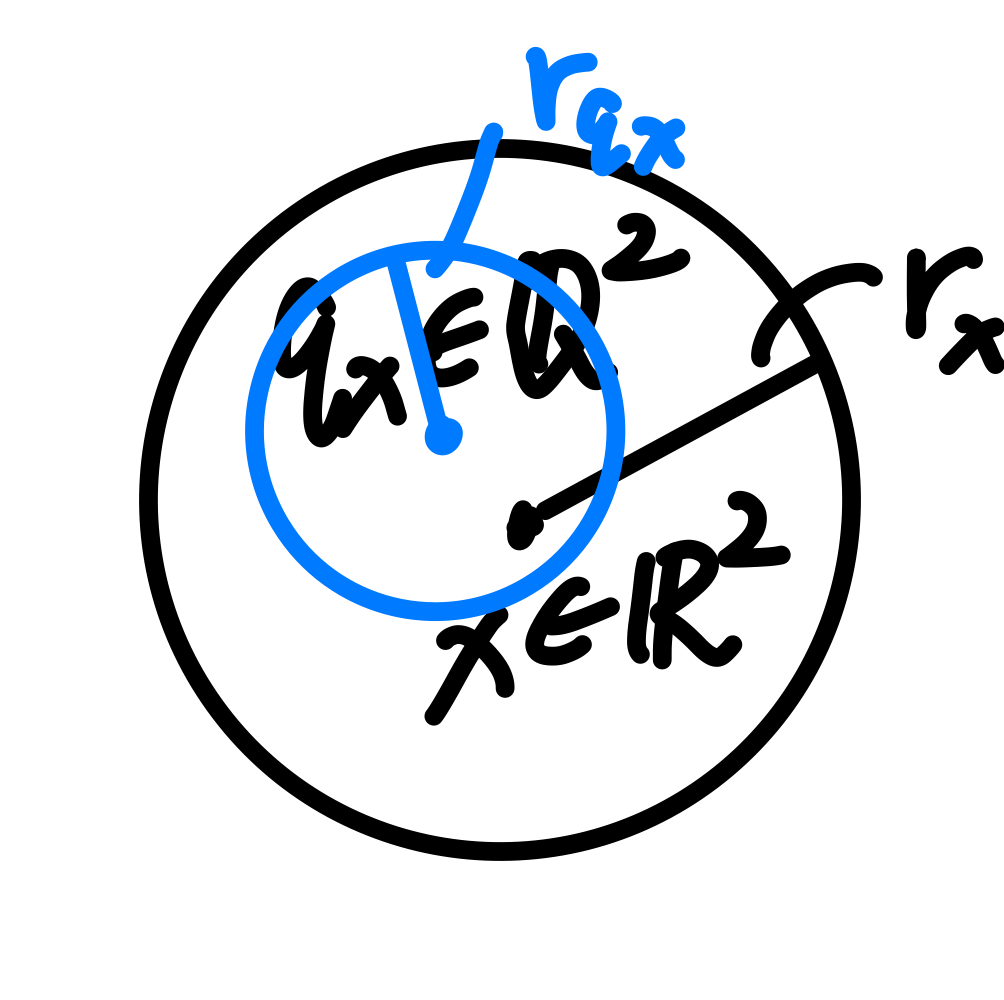
\includegraphics[width=0.2\linewidth,height=\textheight,keepaspectratio]{assets/main--figure-raster-001.png}

\end{center}

For each \(q \in {\mathbb{Q}}_{U}\), we define:

\[r_{q,sup} := \sup\left\{ {r_{q_{x}} \mid q\ \text{is chosen by}\ x} \right\}\]

Now we have:

\[U \subset \bigcup\limits_{q \in U_{q}}B_{r_{q,sup}}(q)\]

This is because for each each \(x \in U\), \(x \in B_{r_{q_{x}}}(q_{x}) \subset B_{r_{q_{x},sup}}(q_{x})\)

And we also have the other direction:

\[\bigcup\limits_{q \in U_{q}}B_{r_{q,sup}}(q) \subseteq U\]

since every \(B_{r_{q}}(q)\) is guaranteed to be the subset of some ball around some \(x \in U\). All togethe we have

\[U = \bigcup\limits_{q \in U_{q}}B_{r_{q,sup}}(q)\]

This finishes the proof of claim 1.

\textbf{Claim 2: every open ball centered at some \(q \in {\mathbb{Q}}^{2}\) is a countable union of admissible annulises with the same center, together with another admissible annulis whose center is also rational.} Proof for Claim 2: Let \(q = (a,b) \in {\mathbb{Q}}^{2}\).\\
We have

\[B(q,R)\backslash\left\{ q \right\} = \bigcup\limits_{n = 1}^{\infty}\left\{ {(x,y):(R - \frac{1}{n})^{2} < (x - a)^{2} + (y - b)^{2} < R^{2}} \right\}\]

-1, 这里写的略有问题, 因为 \(R\) 不一定是 rational 的, 不过我们可以用 density of \(\mathbb{Q}\) in \(\mathbb{R}\) 来写. It remains to cover the center. Let \(q' := (a',b') \in {\mathbb{Q}}^{2}\) such that \(\left. R/6 < \middle| q' - q \middle| < R/3 \right.\), \(r' := R/6\) and \(R' := R/2\) . Then the annuli \(A(a',b',r',R')\) defined by the four parameters is contained in the \(B(q,R)\) and it covers \(\left\{ q \right\}\). Therefore

\[B(q,R) = (\bigcup\limits_{n = 1}^{\infty}\left\{ {(x,y):(R - \frac{1}{n})^{2} < (x - a)^{2} + (y - b)^{2} < R^{2}} \right\}) \cup A(a',b',r',R')\]

\begin{center}

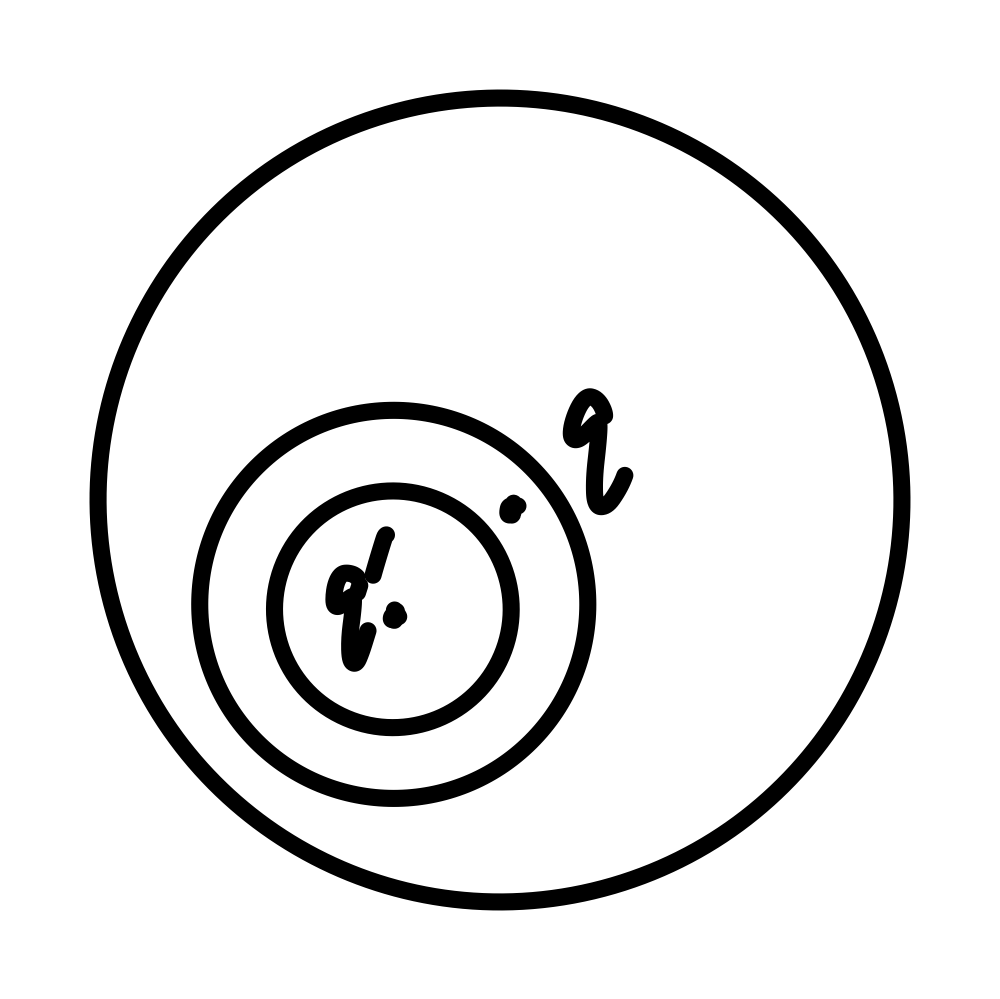
\includegraphics[width=0.2\linewidth,height=\textheight,keepaspectratio]{assets/main--figure-raster-002.png}

\end{center}

This finishes the proof of Claim 2.\\
Combining Claim 1 and Claim 2, we can conclude that \textbf{every open subset of \({\mathbb{R}}^{2}\) is a countable union of admissible annuli.}

\end{proof}

(3)

\begin{proof}

As defined,

\[\mathcal{B}({\mathbb{R}}^{2}) = < \mathcal{T}_{metric} > = < \left\{ {\text{all open sets in}\ {\mathbb{R}}^{2}} \right\} >\]

Let

\[A := \left\{ {\text{all admissible annulis in}\ {\mathbb{R}}^{2}} \right\}\]

Every admissible annuli is open in \({\mathbb{R}}^{2}\), so

\[A \subset \left\{ {\text{all open sets in}\ {\mathbb{R}}^{2}} \right\}\]

and since \(\mathcal{B}({\mathbb{R}}^{2})\) is a \(\sigma\)-algebra, we have

\[< A > \subset < \left\{ {\text{all open sets in}\ {\mathbb{R}}^{2}} \right\} > = \mathcal{B}({\mathbb{R}}^{2})\]

by the proposition proved in class. And by (2), any open set is a countable union of admissible annulis, therefore every open set is in \(< A >\) since any countable union of sets in a \(\sigma\)-algebra is still in the set. So

\[\left\{ {\text{all open sets in}\ {\mathbb{R}}^{2}} \right\} \subset < A >\]

This finishes the proof that

\[< A > = < \left\{ {\text{all open sets in}\ {\mathbb{R}}^{2}} \right\} > = \mathcal{B}({\mathbb{R}}^{2})\]

\end{proof}

\section{Nur für Verrückte}\label{nur-fuxfcr-verruxfcckte}

(It's really not necessary to attempt these problems. Do not hand them in!)

\begin{itemize}
\item
  Let \(X\) be a set, and define two operations on \(\mathcal{P}(X)\):

  \begin{itemize}
  \item
    The ``product'' of two subsets \(E,F \subset X\) is the intersection \(E \cap F\).
  \item
    The ``sum'' of two sets \(E,F \subset X\) is the symmetric difference \(E\Delta F\).
  \item
    Prove that these operations endow \(\mathcal{P}(X)\) with the structure of a commutative ring. What are the additive and multiplicative units? Prove that this ring is idempotent.
  \item
    Let us say that a nonempty subset \(A \subset \mathcal{P}(X)\) is a ring if it is closed under differences and finite unions. In other words, if \(E,F \in A\), then \(E\backslash F \in A\) and \(E \cup F \in A\). Prove that a subset \(A \subset \mathcal{P}(X)\) is an algebra iff it is a ring containing \(X\).
  \item
    Prove that a nonempty subset \(A \subset \mathcal{P}(X)\) is a ring iff it is a subring of \(\mathcal{P}(X)\). Also prove that it is an algebra iff it is a subring containing the multiplicative identity.
  \end{itemize}
\item
  Let \((X,\mathcal{A})\) and \((Y,\mathcal{B})\) be measurable spaces. Say that a map \(f:X\rightarrow Y\) is measurable (with respect to the \(\sigma\)-algebras \(\mathcal{A}\) and \(\mathcal{B}\)) if \(f^{- 1}(E) \in \mathcal{A}\) for every \(E \in \mathcal{B}\).

  \begin{itemize}
  \item
    Prove that measurable spaces with measurable maps as morphisms form a category.
  \item
    Try convincing an analyst that (a) is useful.
  \end{itemize}
\end{itemize}
\end{document}
